\documentclass[journal,12pt,twocolumn]{IEEEtran}
%
\usepackage{setspace}
\usepackage{textcomp}
\usepackage{gensymb}
\usepackage{xcolor}
\usepackage{caption}
\singlespacing

\usepackage[cmex10]{amsmath}
\usepackage{mathtools}
\usepackage{hyperref}
\usepackage{amsthm}
\usepackage{mathrsfs}
\usepackage{txfonts}
\usepackage{stfloats}
\usepackage{cite}
\usepackage{cases}
\usepackage{subfig}
\usepackage{longtable}
\usepackage{multirow}
\usepackage{enumitem}
\usepackage{listings}
\usepackage{graphicx}
\usepackage{amssymb}
\usepackage{siunitx}
\let\vec\mathbf

\DeclareMathOperator*{\Res}{Res}
\renewcommand\thesection{\arabic{section}}
\renewcommand\thesubsection{\thesection.\arabic{subsection}}
\renewcommand\thesubsubsection{\thesubsection.\arabic{subsubsection}}
\renewcommand\thesectiondis{\arabic{section}}
\renewcommand\thesubsectiondis{\thesectiondis.\arabic{subsection}}
\renewcommand\thesubsubsectiondis{\thesubsectiondis.\arabic{subsubsection}}
\hyphenation{op-tical net-works semi-conduc-tor}

\lstset{
language=Python,
frame=single, 
breaklines=true,
columns=fullflexible
}


\usepackage{tikz}
\usetikzlibrary{shapes, arrows, positioning}
\usepackage[RPvoltages]{circuitikz}


\begin{document}
%

\theoremstyle{definition}
\newtheorem{theorem}{Theorem}[section]
\newtheorem{problem}{Problem}
\newtheorem{proposition}{Proposition}[section]
\newtheorem{lemma}{Lemma}[section]
\newtheorem{corollary}[theorem]{Corollary}
\newtheorem{example}{Example}[section]
\newtheorem{definition}{Definition}[section]
\newcommand{\define}{\stackrel{\triangle}{=}}
\newcommand{\myvec}[1]{\ensuremath{\begin{pmatrix}#1\end{pmatrix}}}
\newcommand{\mydet}[1]{\ensuremath{\begin{vmatrix}#1\end{vmatrix}}}
\newcommand\numberthis{\addtocounter{equation}{1}\tag{\theequation}}
\newcommand\intinf{\int_{-\infty}^\infty}


\bibliographystyle{IEEEtran}

\providecommand{\nCr}[2]{\,^{#1}C_{#2}} % nCr
\providecommand{\nPr}[2]{\,^{#1}P_{#2}} % nPr
\providecommand{\mbf}{\mathbf}
\providecommand{\pr}[1]{\ensuremath{\Pr\left(#1\right)}}
\providecommand{\qfunc}[1]{\ensuremath{Q\left(#1\right)}}
\providecommand{\sbrak}[1]{\ensuremath{{}\left[#1\right]}}
\providecommand{\lsbrak}[1]{\ensuremath{{}\left[#1\right.}}
\providecommand{\rsbrak}[1]{\ensuremath{{}\left.#1\right]}}
\providecommand{\brak}[1]{\ensuremath{\left(#1\right)}}
\providecommand{\lbrak}[1]{\ensuremath{\left(#1\right.}}
\providecommand{\rbrak}[1]{\ensuremath{\left.#1\right)}}
\providecommand{\cbrak}[1]{\ensuremath{\left\{#1\right\}}}
\providecommand{\lcbrak}[1]{\ensuremath{\left\{#1\right.}}
\providecommand{\rcbrak}[1]{\ensuremath{\left.#1\right\}}}
\providecommand{\rect}[1]{\text{rect}\ensuremath{\left(#1\right)}}
\providecommand{\sinc}[1]{\text{sinc}\ensuremath{\left(#1\right)}}
\theoremstyle{remark}
\newtheorem{rem}{Remark}
\newcommand{\sgn}{\mathop{\mathrm{sgn}}}
\providecommand{\abs}[1]{\left\vert#1\right\vert}
\providecommand{\res}[1]{\Res\displaylimits_{#1}} 
\providecommand{\norm}[1]{\lVert#1\rVert}
\providecommand{\mtx}[1]{\mathbf{#1}}
\providecommand{\mean}[1]{E\left[ #1 \right]}
\providecommand{\fourier}{\overset{\mathcal{F}}{ \rightleftharpoons}}
\providecommand{\ztrans}{\overset{\mathcal{Z}}{ \rightleftharpoons}}

\providecommand{\system}[1]{\overset{\mathcal{#1}}{ \longleftrightarrow}}
\newcommand{\solution}{\noindent \textbf{Solution: }}
\providecommand{\dec}[2]{\ensuremath{\overset{#1}{\underset{#2}{\gtrless}}}}
\numberwithin{equation}{section}
\makeatletter
\@addtoreset{figure}{problem}
\makeatother

\let\StandardTheFigure\thefigure
\renewcommand{\thefigure}{\theproblem}


\vspace{3cm}

\title{Fourier Series}
\author{Sumanth N R}
\maketitle
\tableofcontents

\renewcommand{\thefigure}{\theenumi}
\renewcommand{\thetable}{\theenumi}

\bigskip

\begin{abstract}
This manual provides a simple introduction to Fourier Series
\end{abstract}


\section{Periodic Function}
Let 
\begin{align}
	x(t) &= A_0\abs{\sin\brak{2\pi f_0 t}}
	\label{eq:10-orig-diff-def}
\end{align}

\begin{enumerate}[label=\thesection.\arabic*, ref=\thesection.\theenumi]

\item Plot $x(t)$. \\
	\solution\\
	The following code yields the graph
	\begin{lstlisting}
wget https://raw.githubusercontent.com/Sigma1084/EE3900/master/charger/codes/Ex1_1_plotxt.py
	\end{lstlisting}
	\begin{figure}[!htp]
		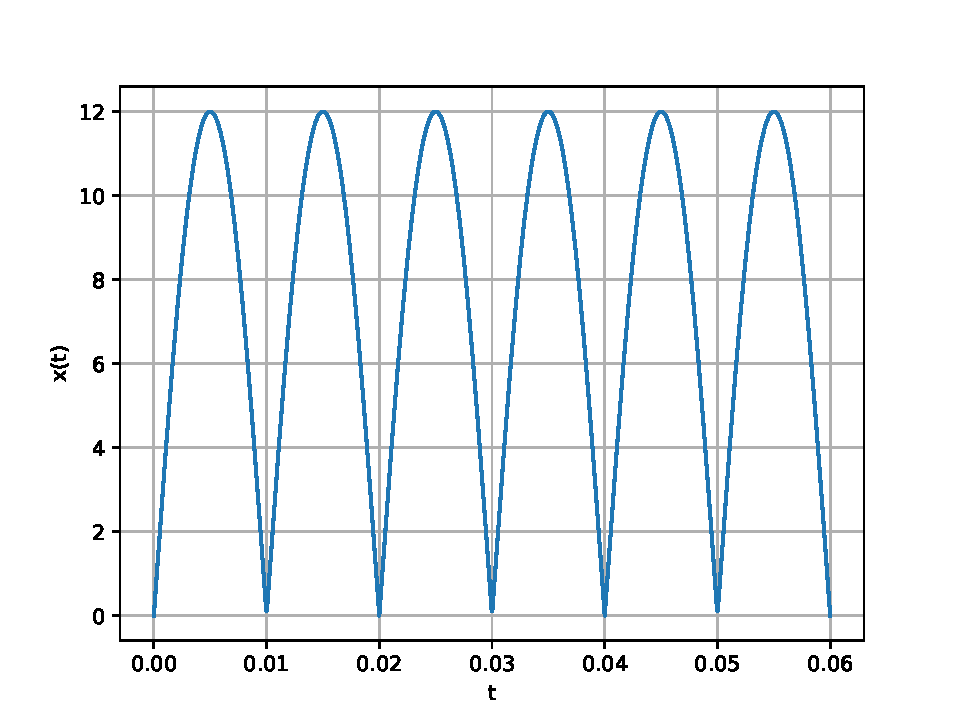
\includegraphics[width=\columnwidth]{figs/Ex1_1_xt}
		\caption{Plot of $x(t)$}
		\label{fig:x-t}
	\end{figure}


\item Show that $x(t)$ is periodic and find its period.
	\solution\\
	We know that \( |\sin(x)| \) is periodic with fundamental period of \( \pi \). \\
	\( \implies \) Fundamental period of \( A|\sin(ax) \) is \( \frac{\pi}{a} \) \\
	Fundamental period of \( A_0|\sin(2\pi f_0 t)| \) is \( \frac{\pi}{2\pi f_0} \) \\
	\( \implies \) Fundamental period of \( x(t) \) is \( \frac{1}{2f_0} \)
	

\end{enumerate}


\section{Fourier Series}

Consider $A_0 =12$ and $f_0 = 50$ for all numerical calculations.

\begin{enumerate}[label=\thesection.\arabic*,ref=\thesection.\theenumi]

\item If
	\begin{align}
		x(t) = \sum_{k = -\infty}^{\infty}c_k e^{j2\pi kf_0 t}
	\label{eq:one-Z-complex}
	\end{align}
	show that
	\begin{align}
		c_k = f_0\int_{-\frac{1}{2f_0}}^{\frac{1}{2f_0}}x(t)e^{-j2\pi kf_0 t}\, dt
	\label{eq:one-Z}
	\end{align}
	\solution\\
	Consider for some \( n \in \mathbb{Z} \),
	\[ x(t) e^{j2\pi nf_0 t} = \sum_{k=-\infty}^\infty c_k e^{j2\pi (k-n) f_0 t} \]
	We know using the periodicity of \( e^{j2\pi kf_0 t} \),
	\[
		\int_{-\frac{1}{2f_0}}^{\frac{1}{2f_0}} e^{j2\pi kf_0 t} dt =
		\begin{cases}
			\frac{1}{f_0} \text{ if } k=0 \\
			0 \text{ otherwise}
		\end{cases}
	\]
	Now,
	\begin{align*}
		\int_{-\frac{1}{2f_0}}^{\frac{1}{2f_0}}x(t) e^{j2\pi nf_0 t} dt
		&= \int_{-\frac{1}{2f_0}}^{\frac{1}{2f_0}}
		\sum_{k=-\infty}^\infty c_k e^{j2\pi (k-n) f_0 t} \\
		&= \frac{c_n}{f_0}
	\end{align*}
	\[
		\implies c_n = f_0 \int_{-\frac{1}{2f_0}}^{\frac{1}{2f_0}}x(t) e^{j2\pi nf_0 t} dt
	\]
	
	\pagebreak

\item
	Find $c_k$ for~\eqref{eq:10-orig-diff-def} \\
	\solution
	\begin{align*}
		c_k &= f_0 \int_{-\frac{1}{2f_0}}^{\frac{1}{2f_0}}x(t) e^{j2\pi kf_0 t} dt \\
		&= f_0 \int_{-\frac{1}{2f_0}}^{\frac{1}{2f_0}}
			A_0\abs{\sin\brak{2\pi f_0 t}} e^{j2\pi kf_0 t} dt \\
		&= f_0 \int_{-\frac{1}{2f_0}}^{\frac{1}{2f_0}}
			A_0\abs{\sin\brak{2\pi f_0 t}}
			\cos(2\pi kf_0 t) dt \\
		& \quad + jf_0 \int_{-\frac{1}{2f_0}}^{\frac{1}{2f_0}}
			A_0\abs{\sin\brak{2\pi f_0 t}}
			\sin(2\pi kf_0 t) dt \\
		&= f_0 \int_{-\frac{1}{2f_0}}^{\frac{1}{2f_0}}
			A_0\abs{\sin\brak{2\pi f_0 t}}
			\cos(2\pi kf_0 t) dt + 0 \\
		&= 2f_0 \int_{0}^{\frac{1}{2f_0}}
			A_0\sin\brak{2\pi f_0 t}
			\cos(2\pi kf_0 t) dt \\
		&= f_0 A_0 \int_{0}^{\frac{1}{2f_0}} \sin \brak{2\pi\brak{n+1}f_0 t} dt \\
		& \quad - f_0 A_0\int_{0}^{\frac{1}{2f_0}}\sin\brak{2\pi\brak{n-1}f_0 t} dt \\
		&= f_0 A_0\frac{1+\brak{-1}^n}{2\pi f_0}\brak{\frac{1}{n+1} - \frac{1}{n-1}} \\
		&= 
		\begin{cases}
			\frac{2A_0}{\pi\brak{1-n^2}} & n\ \text{even} \\
			0 & n\ \text{odd}
		\end{cases} \numberthis \label{eq:ck}
	\end{align*}


\item Verify~\eqref{eq:10-orig-diff-def} and~\eqref{eq:one-Z-complex} using python. \\
	\solution
	The following code yields the graph
	\begin{lstlisting}
wget https://raw.githubusercontent.com/Sigma1084/EE3900/master/charger/codes/Ex2_3_verify_xt.py
	\end{lstlisting}
	\begin{figure}[!ht]
    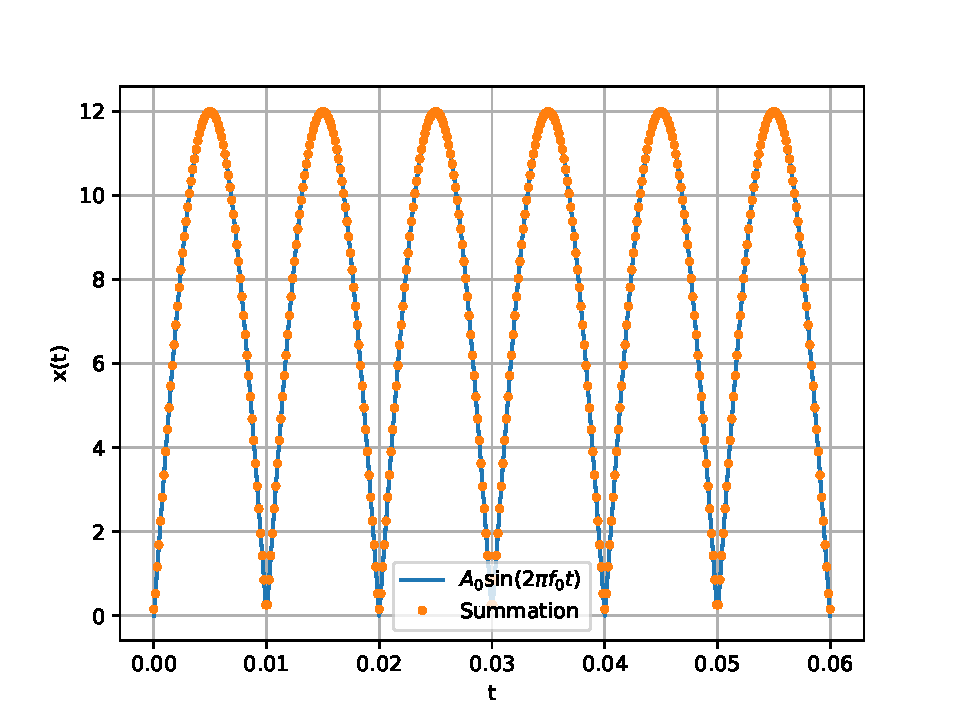
\includegraphics[width=\columnwidth]{figs/Ex2_3_verify_xt}
		\caption{Verification of~\eqref{eq:one-Z-complex}.}
		\label{fig:verify_xt}
	\end{figure}
	

\item Show that 
	\begin{align}
		x(t) = \sum_{k = 0}^{\infty}\brak{a_k\cos{j2\pi kf_0 t}+b_k\sin{j2\pi kf_0 t}}
	\label{eq:one-Z-real}
	\end{align}
	and obtain the formulae for $a_k$ and $b_k$. \\
	\solution\\
	\solution From~\eqref{eq:one-Z-complex},
	\begin{align*}
		x(t) &= \sum_{k = -\infty}^{\infty}c_k e^{j2\pi kf_0 t} \\
		&= c_0 + \sum_{k = 1}^{\infty} \brak{c_k e^{j2\pi kf_0 t} + c_{-k}e^{-j2\pi kf_0 t}} \\
		&= c_0 + \sum_{k = 1}^{\infty} \brak{c_k + c_{-k}}\cos\brak{2\pi kf_0 t} \\
		& \quad + j\sum_{k = 0}^{\infty}\brak{c_k - c_{-k}}\sin\brak{2\pi kf_0 t}
	\end{align*}
	Hence, for \( k \ge 0 \),
	\begin{align}
		a_k &= 
		\begin{cases}
			c_0 & k = 0 \\
			c_k + c_{-k} & k > 0
		\end{cases}
		\label{eq:ak} \\
		b_k &= j \brak{c_k - c_{-k}}
		\label{eq:bk}
	\end{align}
	

\item Find $a_k$ and $b_k$ for~\eqref{eq:10-orig-diff-def} \\
	\solution \\
	Using the expression for \( c_k \), from~\eqref{eq:ck} \\
	and using~\eqref{eq:ak} and~\eqref{eq:bk}, we have,
	\begin{align*}
		a_k &= 
			\begin{cases}
				\frac{2A_0}{\pi} & k = 0 \\
				\frac{4A_0}{\pi\brak{1-k^2}} & k \text{ even} \\
				0 & k \text{ odd}
			\end{cases} \\
		b_k &= 0
	\end{align*}

\pagebreak

\item Verify~\eqref{eq:one-Z-real} using python \\
	\solution \\
	The following code block yields the graph
	\begin{lstlisting}
wget https://raw.githubusercontent.com/Sigma1084/EE3900/master/charger/codes/Ex2_3_verify_xt_real.py
	\end{lstlisting}
	\begin{figure}[!ht]
	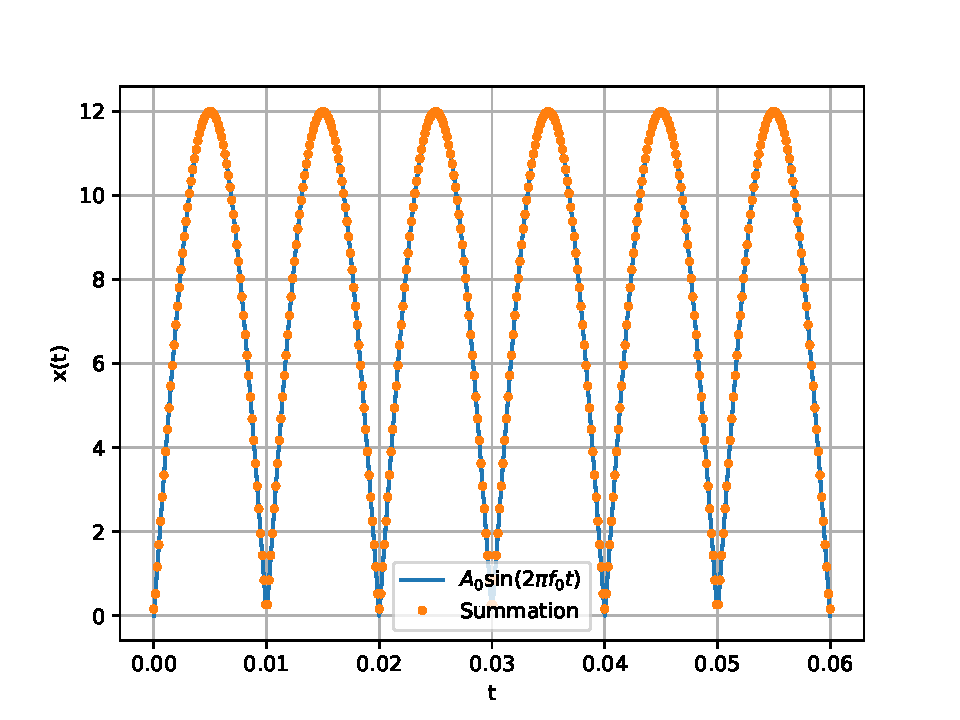
\includegraphics[width=\columnwidth]{figs/Ex2_4_verify_xt_real}
		\caption{Verification of~\eqref{eq:one-Z-real}.}
		\label{fig:verify_xt_real}
	\end{figure}

\end{enumerate}



\section{Fourier Transform}
\begin{enumerate}[label=\thesection.\arabic*, ref=\thesection.\theenumi]

\item 
	\begin{align}
		\delta(t)&=0, \quad t\neq0 \\
		\int_{-\infty}^{\infty}\delta(t) \, dt&= 1
	\end{align}

\item The Fourier Transform of $g(t)$ is
	\begin{align}
		G(f)=\int_{-\infty}^{\infty}g(t)e^{-j2\pi ft}\,dt
	\end{align}


\item Show that 
	\begin{align}
		g(t-t_0)&\system{F}G(f)e^{-j2\pi ft_0}
	\end{align}
	\solution
	\begin{align*}
		\mathcal{F}\brak{g\brak{t-t_0}} &= \int_{-\infty}^\infty g\brak{t-t_0} e^{-j2\pi ft} dt \\
		&= \int_{-\infty}^\infty g\brak{t} e^{-j2\pi f\brak{t+t_0}} dt \\
		&= e^{-j2\pi ft_0} \int_{-\infty}^\infty g\brak{t} e^{-j2\pi ft} dt \\
		&= G(f) e^{-j2\pi ft_0}
	\end{align*}
	\( \implies g\brak{t-t_0} \system{F} G(f) e^{-j2\pi ft_0} \) \\
	Hence proved


\item Show that 
	\begin{align}
		G(t)&\system{F}g(-f)
	\end{align}
	\solution\\
	Using the definition of inverse Fourier Transform,
	\[ g(t) = \int_{-\infty}^\infty G(f) e^{j2\pi ft} df \]
	Now, putting \( -f \coloneqq t, \ t \coloneqq f \implies df = dt \), \\
	\begin{gather*}
	    g(-f) = \int_{-\infty}^\infty G(t) e^{-j2\pi ft} dt\\
	    \implies G(t) \system{F} g(-f) \numberthis \label{eq:G-to-g}\\
	\end{gather*}


\item $\delta(t)\system{F}?$ \\
	\solution
	\begin{align*}
		\delta(t) \system{F} & \intinf \delta(t) e^{-j2\pi ft} dt \\
			&= e^{-j2 \pi f(0)} \intinf \delta(t) dt \\
		\delta(t) \system{F} & 1 \numberthis \label{eq:fourier-delta}
	\end{align*}


\item $e^{-j2\pi f_0 t}\system{F}?$ \\
	\solution Suppose \( g(t) \system{F} G(f) \)
	\begin{align*}
		g(t) e^{-j2\pi f_0 t} \system{F} & \intinf g(t) e^{-j2 \pi \brak{f_0 + f} t} dt \\
		&= G(f + f_0)
	\end{align*}
	Now, using~\eqref{eq:fourier-delta} and~\eqref{eq:G-to-g} , we can get,
	\[ \delta(t) \system{F} 1 \system{F} \delta(-t) \]
	Putting \( g(t) = 1 \) and hence, \( G(f) = \delta(-f) = \delta(f) \), 
	we get \( G(f + f_0) = \delta(f+f_0) \).
	Hence,
	\[ e^{-j2\pi f_0 t} \system{F} \delta(f+f_0) \numberthis \label{eq:fourier-exp} \]


\item $\cos(2\pi f_0 t)\system{F}?$ \\
	\solution We can write
	\[ \cos(2\pi f_0 t) = \frac{1}{2} \brak{e^{j2\pi f_0 t} + e^{-j2\pi f_0 t}} \]
	Using \eqref{eq:fourier-exp} and the linearity of Fourier Transform, we get,
	\[ \cos(2\pi f_0 t) \system{F} \frac{1}{2}\Big{(} \delta(f-f_0) + \delta(f+f_0) \Big{)} \]


\item Find the Fourier Transform of $x(t)$ and plot it.
	Verify using python. \\
	\solution
	Using~\eqref{eq:one-Z-complex}, we have,
	\[ x(t) = \sum_{k = -\infty}^{\infty}c_k e^{j2\pi kf_0 t} \]
	Using~\eqref{eq:fourier-exp}, we get,
	\begin{align*}
		x(t) \system{F} & \sum_{k=-\infty}^\infty c_k \delta(f-kf_0) \\
		&= \frac{2A_0}{\pi} \sum_{k=-\infty}^\infty \frac{\delta(f-2kf_0)}{1-4k^2} \\
	\end{align*}
	\begin{lstlisting}
wget https://raw.githubusercontent.com/Sigma1084/EE3900/master/charger/codes/Ex3_08_x-fourier.py
	\end{lstlisting}
	\begin{figure}[h]
		\centering
		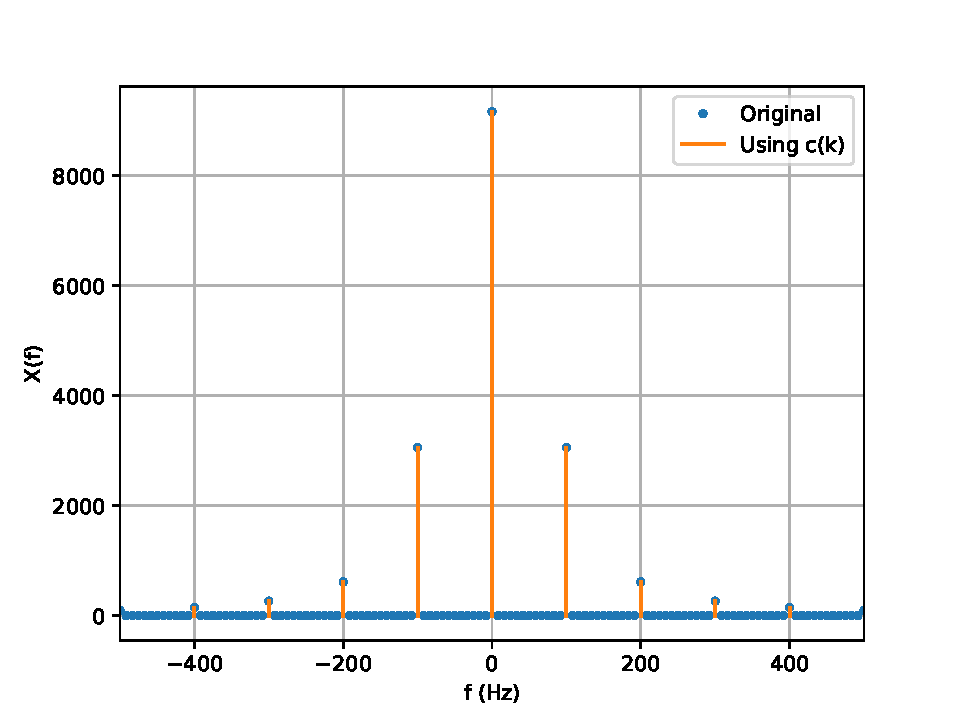
\includegraphics[width=0.5\textwidth]{figs/Ex3_08_verify_xt_fourier}
		\caption{Fourier Transform of $x(t)$}
		\label{fig:verify_xt_fourier}
	\end{figure}
	

\item Show that
	\begin{align}
		\rect{t} \system{F} \sinc{t}
		\label{eq:rect-to-sinc}
	\end{align}
	Verify using python. \\
	\solution
	\begin{align*}
		\rect{t} \system{F} & \intinf \rect{t} e^{-j2\pi ft} dt \\
		&= \int_{-\frac{1}{2}}^{\frac{1}{2}} e^{-j2\pi ft} dt \\
		&= \frac{1}{-j2\pi f} \brak{e^{-j\pi f} - e^{j\pi f}} \\
		&= \frac{\sin(\pi f)}{\pi f} = \sinc{f}
	\end{align*}
	\begin{lstlisting}
wget https://raw.githubusercontent.com/Sigma1084/EE3900/master/charger/codes/Ex3_09_rect-fourier.py
	\end{lstlisting}
	\begin{figure}[h]
		\centering
		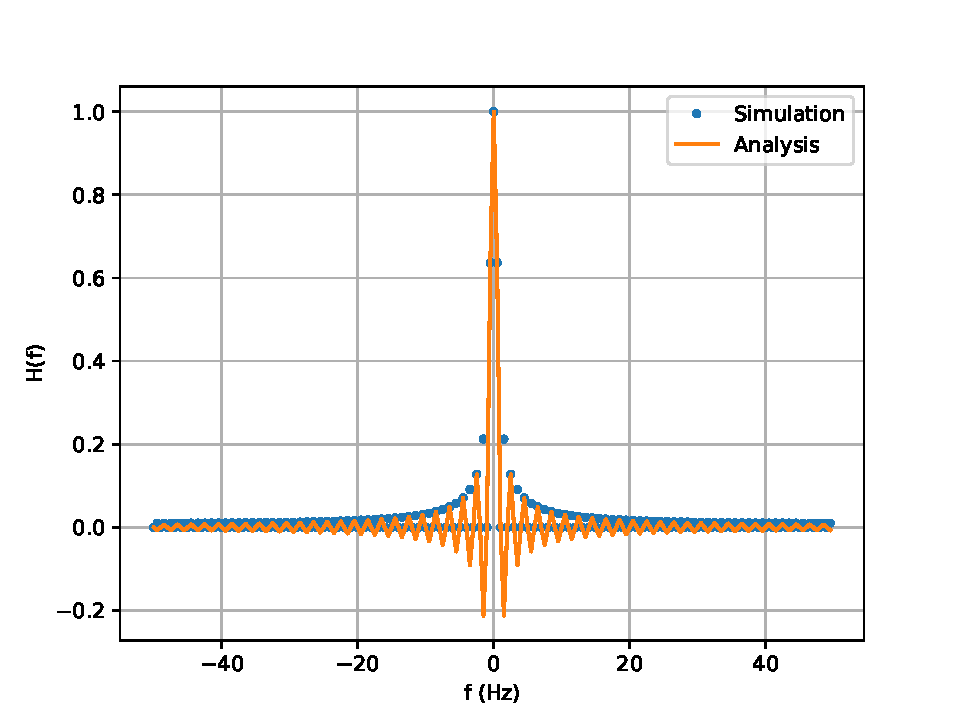
\includegraphics[width=0.5\textwidth]{figs/Ex3_09_verify_rect_fourier}
		\caption{Fourier Transform of $x(t)$}
		\label{fig:verify_rect_fourier}
	\end{figure}


\item 
	$\sinc{t}\system{F} ?$
	Verify using python. \\
	\solution \\
	Using~\eqref{eq:rect-to-sinc}, and~\eqref{eq:G-to-g}, we get,
	\[ \sinc{t} \system{F} \rect{-f} = \rect{f} \numberthis \label{eq:sinc-to-rect} \]
	\begin{lstlisting}
wget https://raw.githubusercontent.com/Sigma1084/EE3900/master/charger/codes/Ex3_10_sinc-fourier.py
	\end{lstlisting}
	\begin{figure}[h]
		\centering
		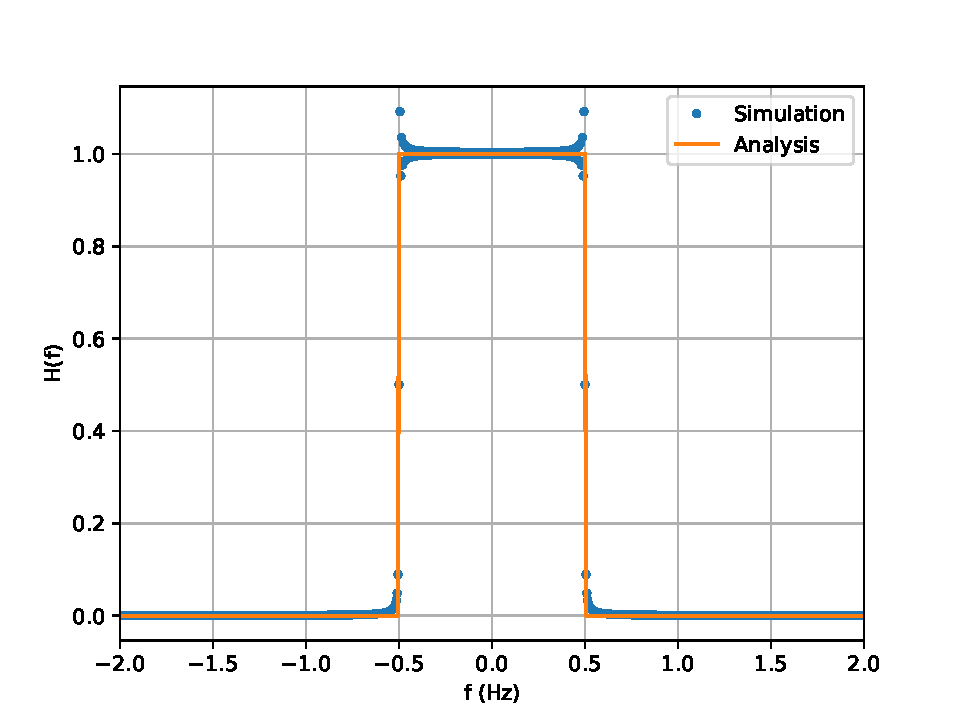
\includegraphics[width=0.5\textwidth]{figs/Ex3_10_verify_sinc_fourier}
		\caption{Fourier Transform of $x(t)$}
		\label{fig:verify_sinc_fourier}
	\end{figure}

\end{enumerate}



\section{Filter}
\begin{enumerate}[label=\thesection.\arabic*, ref=\thesection.\theenumi]


\item Find $H(f)$ which transforms $x(t)$ to DC 5V. \\
\solution The function $H(f)$ is a low pass filter which filters out
even harmonics and leaves the zero frequency component behind.
The rectangular function represents an ideal low pass filter.
Suppose the cutoff frequency is $f_c = 50$ Hz, then
\begin{align}
    H(f) = \rect{\frac{f}{2f_c}} =
    \begin{cases}
        1 & \abs{f} < f_c \\
        0 & \textrm{otherwise}
    \end{cases}
    \label{eq:Hf}
\end{align}
Multiplying by a scaling factor to get DC 5V,
\begin{align*}
    H(f) = \frac{\pi V_0}{2A_0}\rect{\frac{f}{2f_c}}
\end{align*}
where $V_0 = 5$ V\@.

\item Find $h(t)$. \\
\solution Suppose $g(t)\system{F}G(f)$.
Then, for some nonzero $a \in \mathbb{R}$
\begin{align*}
	g(at)&\system{F}\int_{-\infty}^{\infty}g(at)e^{-j2\pi ft}\, dt \\
	&=\frac{1}{a}\int_{-\infty}^{\infty}g(u)e^{\brak{-j2\pi \frac{f}{a}t}}\, dt \\
	&=\frac{1}{a}G\brak{\frac{f}{a}}
	\label{eq:t-scaling}
\end{align*}
where we have substituted $u \coloneqq at$.
\begin{align*}
    \therefore h(t) = \frac{2\pi V_0}{A_0}f_c\sinc{2f_c t}
\end{align*}


\item Verify your result using  through convolution.
\solution
	Fourier transform of $x(t)$ and $h(t)$ respectively is
	\begin{align}
		X(f)&=\sum_{k=-\infty}^{\infty} \frac{2A_0}{\pi} \frac{\delta\brak{f+2kf_0}}{1-4k^2}\\
		H(f)&=\frac{\pi V_0}{2A_0}\rect{\brak{\frac{f}{2f_c}}}\\
		X(f) \times H(f)&=\sum_{k=-\infty}^{\infty} V_0 \frac{\delta\brak{f+2kf_0}}{1-4k^2} \times \rect{\brak{\frac{f}{2f_c}}}\\
		X(f)\times H(f)&=\sum_{k=0}^{0} V_0 \frac{\delta\brak{f+2kf_0}}{1-4k^2}
	\end{align}
	Hence,
	\begin{align}
		X(f)\times H(f)&=V_0 \frac{\delta\brak{f}}{1-4 \times 0}\\
		X(f)\times H(f)&=V_0 \delta\brak{f}
	\end{align}
Since $1\system{F} \delta\brak{0}$,
Hence,
\begin{align}
	V_0 \delta\brak{t} \system{F} V_0\times 1 \\
	\implies H(t) \circledast x(t)=V_0
\end{align}
Hence verified.
\begin{figure}[!ht]
	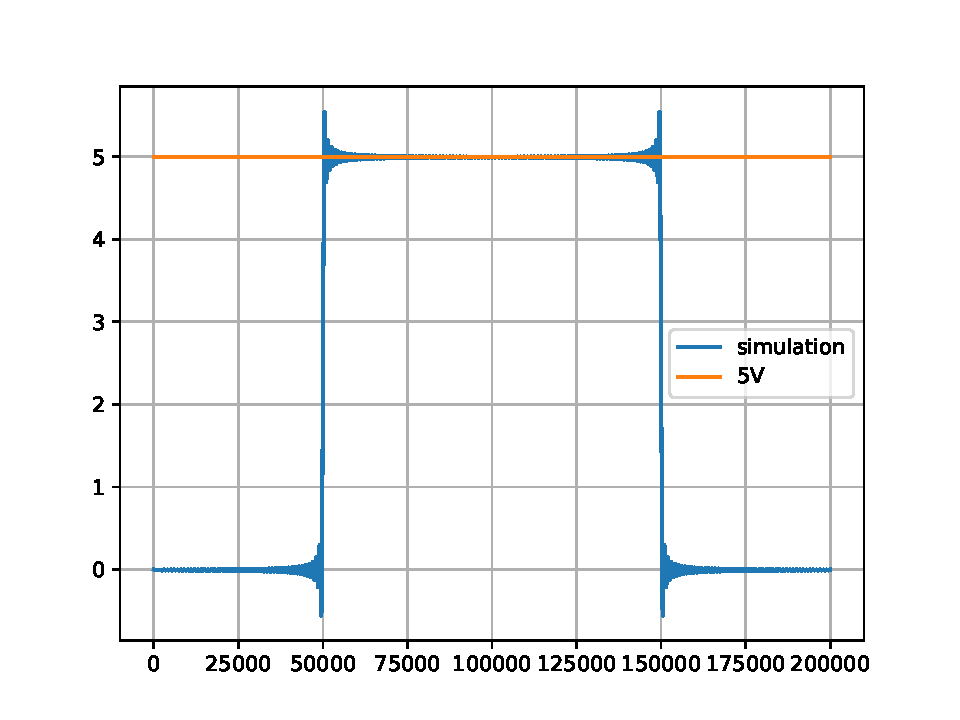
\includegraphics[width=\columnwidth]{figs/Ex4_convolution}
	\caption{Convolution of the $x(t)$ and $h(t)$.}
	\label{fig:convolution}
\end{figure}
The following python yields the plot~\ref{fig:convolution}.
\begin{lstlisting}
wget https://raw.githubusercontent.com/Sigma1084/EE3900/master/charger/codes/Ex4_convolution.py
\end{lstlisting}


\end{enumerate}

\section{Filter Design}

\begin{enumerate}[label=\thesection.\arabic*, ref=\thesection.\theenumi]

\item Design a Butterworth filter for $H(f)$

	\solution The transfer function of a Butterworth filter is given by
	\begin{align}
		\abs{H_n(f)} = \frac{1}{\sqrt{1+\brak{\frac{f}{f_c}}^{2n}}}
	\end{align}
	where $n$ is the order of the filter and $f_c$ is the cutoff frequency

	Let the passband and stopband frequency thresholds be $\SI{50}{\hertz}$ and $\SI{100}{\hertz}$ and their corresponding attenuations be $-\SI{1}{\decibel}$ and $-\SI{5}{\decibel}$ respectively
	\begin{align}
		A_p &= 10 \log_{10}\abs{H_n(f_p)}^2 \\
		&= -10\log_{10}\brak{1+\brak{\frac{f_p}{f_c}}^{2n}} \\
		A_s &= -10\log_{10}\brak{1+\brak{\frac{f_s}{f_c}}^{2n}} \\
		\implies n &=\frac{\log\brak{\frac{10^{-\frac{A_p}{10}}-1}{ 10^{-\frac{A_s}{10}}-1}}}{2 \log \brak{\frac{f_p}{f_s}}} \approx 1.53
	\end{align}

	Hence, we choose a $2^{\mathrm{nd}}$ order Butterworth filter with
	\begin{align}
		f_c = \frac{f_p}{\brak{10^{-\frac{A_p}{10}}-1}^{\frac{1}{2n}}} \approx \SI{77.74}{\hertz}
	\end{align}

\item Design a Chebyschev filter for $H(f)$

	\solution The transfer function of a Chebyshev filter is given by
	\begin{align}
		\abs{H_n(f)} =\frac{1}{\sqrt{1+\epsilon^{2}T_{n}^2\brak{\frac{f}{f_c}}}}
	\end{align}
	where $\epsilon$ is the ripple factor, $f_c$ is the cutoff frequency and $T_n$ is a Chebyshev polynomial of the $n^{\mathrm{th}}$ order

	Assuming the same parameters as before along with a ripple of $\SI{0.1}{\decibel}$, we get
	\begin{align}
		\epsilon = \sqrt{10^{\frac{\delta}{10}} - 1} \approx 0.15
	\end{align}

	Also, assume that $f_c = f_p \implies \frac{f_s}{f_c} > 1$
	\begin{align}
		&A_s = -10\log_{10}\brak{1+\epsilon^{2}T_{n}^2\brak{\frac{f_s}{f_c}}} \\
		\implies &T_{n}\brak{\frac{f_s}{f_c}} = \frac{\sqrt{10^{-\frac{A_s}{10}} - 1}}{\epsilon} \\
		\implies &\cosh\brak{n\cosh^{-1}\brak{\frac{f_s}{f_c}}} = \frac{\sqrt{10^{-\frac{A_s}{10}} - 1}}{\epsilon}
	\end{align}

	Thus
	\begin{align}
		n = \frac{\cosh^{-1}\brak{\frac{\sqrt{10^{-\frac{A_s}{10}} - 1}}{\epsilon} }}{\cosh^{-1}\brak{\frac{f_s}{f_c}}} \approx 2.26
	\end{align}

	Hence, we choose a $3^{\mathrm{rd}}$ order Chebyshev filter

\item Design a circuit for your Butterworth filter

	\solution Using the table of normalized Butterworth coefficients, we can see that for a $2^{\mathrm{nd}}$ order Butterworth filter
	\begin{align}
		C_1 &= \SI{1.4142}{\farad} \\
		L_2 &= \SI{1.4142}{\henry}
	\end{align}

	On denormalizing these values, we get
	\begin{align}
		C_1' &= \frac{C_1}{2\pi f_c} = \SI{2.89}{\milli\farad} \\
		L_2' &= \frac{L_2}{2\pi f_c} = \SI{2.89}{\milli\henry}
	\end{align}

	\begin{figure}[!ht]
    \centering
    \begin{circuitikz}
        \draw (0,0) to[short, o-o] (4,0);
        \draw (1,0) to[C, l=\SI{2.89}{\milli\farad}] (1,2);
        \draw (0,2) to [short, o-] (1,2)
        		to [L, l=\SI{2.89}{\milli\henry}] (3.5,2)
        		-- (4,2) to[short, -o] (4,2);
    \end{circuitikz}
    \caption{$2^{\mathrm{nd}}$ order Butterworth filter circuit}
    \label{ckt:butter}
	\end{figure}

\item Design a circuit for your Chebyschev filter

	\solution Using the table of normalized Chebyshev coefficients, we can see that for a $3^{\mathrm{rd}}$ order Chebyshev filter
	\begin{align}
		C_1 &= \SI{1.4328}{\farad} \\
		L_2 &= \SI{1.5937}{\henry} \\
		C_3 &= \SI{1.4328}{\farad}
	\end{align}

	On denormalizing these values, we get
	\begin{align}
		C_1' &= \frac{C_1}{2\pi f_c} = \SI{4.56}{\milli\farad} \\
		L_2' &= \frac{L_2}{2\pi f_c} = \SI{5.07}{\milli\henry} \\
		C_3' &= \frac{C_3}{2\pi f_c} = \SI{4.56}{\milli\farad}
	\end{align}

	\begin{figure}[!ht]
    \centering
    \begin{circuitikz}
        \draw (0,0) to[short, o-o] (5,0);
        \draw (0,2) to [short, o-] (1,2)
        		to [L, l=\SI{5.07}{\milli\henry}] (3.5,2)
        		-- (5,2) to[short, -o] (5,2);
        \draw (1,0) to[C, l=\SI{4.56}{\milli\farad}] (1,2);
        \draw (3.5,0) to[C, l=\SI{4.56}{\milli\farad}] (3.5,2);
    \end{circuitikz}
    \caption{$3^{\mathrm{rd}}$ order Chebyshev filter circuit}
    \label{ckt:cheby}
	\end{figure}

\end{enumerate}


\end{document}
